% Created by tikzDevice version 0.12
% !TEX encoding = UTF-8 Unicode
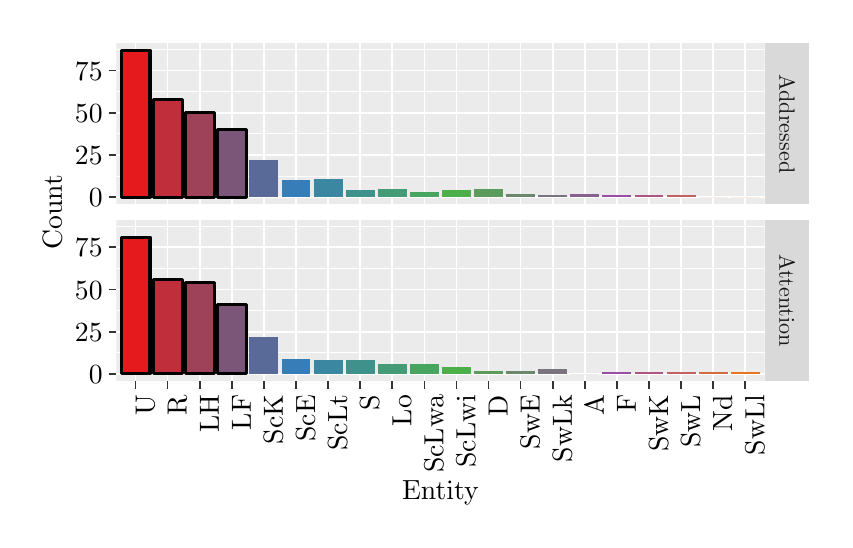
\begin{tikzpicture}[x=1pt,y=1pt]
\definecolor{fillColor}{RGB}{255,255,255}
\path[use as bounding box,fill=fillColor,fill opacity=0.00] (0,0) rectangle (288.00,177.98);
\begin{scope}
\path[clip] (  0.00,  0.00) rectangle (288.00,177.98);
\definecolor{drawColor}{RGB}{255,255,255}
\definecolor{fillColor}{RGB}{255,255,255}

\path[draw=drawColor,line width= 0.6pt,line join=round,line cap=round,fill=fillColor] (  0.00,  0.00) rectangle (288.00,177.98);
\end{scope}
\begin{scope}
\path[clip] ( 32.03,114.10) rectangle (266.25,172.48);
\definecolor{fillColor}{gray}{0.92}

\path[fill=fillColor] ( 32.03,114.10) rectangle (266.25,172.48);
\definecolor{drawColor}{RGB}{255,255,255}

\path[draw=drawColor,line width= 0.3pt,line join=round] ( 32.03,124.38) --
	(266.25,124.38);

\path[draw=drawColor,line width= 0.3pt,line join=round] ( 32.03,139.63) --
	(266.25,139.63);

\path[draw=drawColor,line width= 0.3pt,line join=round] ( 32.03,154.88) --
	(266.25,154.88);

\path[draw=drawColor,line width= 0.3pt,line join=round] ( 32.03,170.14) --
	(266.25,170.14);

\path[draw=drawColor,line width= 0.6pt,line join=round] ( 32.03,116.76) --
	(266.25,116.76);

\path[draw=drawColor,line width= 0.6pt,line join=round] ( 32.03,132.01) --
	(266.25,132.01);

\path[draw=drawColor,line width= 0.6pt,line join=round] ( 32.03,147.26) --
	(266.25,147.26);

\path[draw=drawColor,line width= 0.6pt,line join=round] ( 32.03,162.51) --
	(266.25,162.51);

\path[draw=drawColor,line width= 0.6pt,line join=round] ( 38.99,114.10) --
	( 38.99,172.48);

\path[draw=drawColor,line width= 0.6pt,line join=round] ( 50.58,114.10) --
	( 50.58,172.48);

\path[draw=drawColor,line width= 0.6pt,line join=round] ( 62.18,114.10) --
	( 62.18,172.48);

\path[draw=drawColor,line width= 0.6pt,line join=round] ( 73.77,114.10) --
	( 73.77,172.48);

\path[draw=drawColor,line width= 0.6pt,line join=round] ( 85.37,114.10) --
	( 85.37,172.48);

\path[draw=drawColor,line width= 0.6pt,line join=round] ( 96.96,114.10) --
	( 96.96,172.48);

\path[draw=drawColor,line width= 0.6pt,line join=round] (108.56,114.10) --
	(108.56,172.48);

\path[draw=drawColor,line width= 0.6pt,line join=round] (120.15,114.10) --
	(120.15,172.48);

\path[draw=drawColor,line width= 0.6pt,line join=round] (131.75,114.10) --
	(131.75,172.48);

\path[draw=drawColor,line width= 0.6pt,line join=round] (143.34,114.10) --
	(143.34,172.48);

\path[draw=drawColor,line width= 0.6pt,line join=round] (154.93,114.10) --
	(154.93,172.48);

\path[draw=drawColor,line width= 0.6pt,line join=round] (166.53,114.10) --
	(166.53,172.48);

\path[draw=drawColor,line width= 0.6pt,line join=round] (178.12,114.10) --
	(178.12,172.48);

\path[draw=drawColor,line width= 0.6pt,line join=round] (189.72,114.10) --
	(189.72,172.48);

\path[draw=drawColor,line width= 0.6pt,line join=round] (201.31,114.10) --
	(201.31,172.48);

\path[draw=drawColor,line width= 0.6pt,line join=round] (212.91,114.10) --
	(212.91,172.48);

\path[draw=drawColor,line width= 0.6pt,line join=round] (224.50,114.10) --
	(224.50,172.48);

\path[draw=drawColor,line width= 0.6pt,line join=round] (236.10,114.10) --
	(236.10,172.48);

\path[draw=drawColor,line width= 0.6pt,line join=round] (247.69,114.10) --
	(247.69,172.48);

\path[draw=drawColor,line width= 0.6pt,line join=round] (259.29,114.10) --
	(259.29,172.48);
\definecolor{drawColor}{RGB}{0,0,0}
\definecolor{fillColor}{RGB}{228,26,28}

\path[draw=drawColor,line width= 1.1pt,line join=round,fill=fillColor] ( 33.77,116.76) rectangle ( 44.20,169.83);
\definecolor{fillColor}{RGB}{193,46,59}

\path[draw=drawColor,line width= 1.1pt,line join=round,fill=fillColor] ( 45.36,116.76) rectangle ( 55.80,152.14);
\definecolor{fillColor}{RGB}{158,66,90}

\path[draw=drawColor,line width= 1.1pt,line join=round,fill=fillColor] ( 56.96,116.76) rectangle ( 67.39,147.26);
\definecolor{fillColor}{RGB}{124,86,121}

\path[draw=drawColor,line width= 1.1pt,line join=round,fill=fillColor] ( 68.55,116.76) rectangle ( 78.99,141.16);
\definecolor{fillColor}{RGB}{89,106,152}

\path[fill=fillColor] ( 80.15,116.76) rectangle ( 90.58,130.18);
\definecolor{fillColor}{RGB}{55,126,184}

\path[fill=fillColor] ( 91.74,116.76) rectangle (102.18,122.86);
\definecolor{fillColor}{RGB}{59,135,162}

\path[fill=fillColor] (103.34,116.76) rectangle (113.77,123.47);
\definecolor{fillColor}{RGB}{63,145,139}

\path[fill=fillColor] (114.93,116.76) rectangle (125.37,119.20);
\definecolor{fillColor}{RGB}{68,155,117}

\path[fill=fillColor] (126.53,116.76) rectangle (136.96,119.81);
\definecolor{fillColor}{RGB}{72,165,96}

\path[fill=fillColor] (138.12,116.76) rectangle (148.56,118.59);
\definecolor{fillColor}{RGB}{77,175,74}

\path[fill=fillColor] (149.72,116.76) rectangle (160.15,119.20);
\definecolor{fillColor}{RGB}{92,155,91}

\path[fill=fillColor] (161.31,116.76) rectangle (171.75,119.81);
\definecolor{fillColor}{RGB}{107,136,109}

\path[fill=fillColor] (172.91,116.76) rectangle (183.34,117.98);
\definecolor{fillColor}{RGB}{122,116,127}

\path[fill=fillColor] (184.50,116.76) rectangle (194.94,117.37);
\definecolor{fillColor}{RGB}{137,97,145}

\path[fill=fillColor] (196.10,116.76) rectangle (206.53,117.98);
\definecolor{fillColor}{RGB}{152,78,163}

\path[fill=fillColor] (207.69,116.76) rectangle (218.13,117.37);
\definecolor{fillColor}{RGB}{172,87,130}

\path[fill=fillColor] (219.29,116.76) rectangle (229.72,117.37);
\definecolor{fillColor}{RGB}{193,97,97}

\path[fill=fillColor] (230.88,116.76) rectangle (241.32,117.37);
\definecolor{fillColor}{RGB}{213,107,65}

\path[fill=fillColor] (242.48,116.76) rectangle (252.91,116.76);
\definecolor{fillColor}{RGB}{234,117,32}

\path[fill=fillColor] (254.07,116.76) rectangle (264.51,116.76);
\end{scope}
\begin{scope}
\path[clip] ( 32.03, 50.22) rectangle (266.25,108.60);
\definecolor{fillColor}{gray}{0.92}

\path[fill=fillColor] ( 32.03, 50.22) rectangle (266.25,108.60);
\definecolor{drawColor}{RGB}{255,255,255}

\path[draw=drawColor,line width= 0.3pt,line join=round] ( 32.03, 60.50) --
	(266.25, 60.50);

\path[draw=drawColor,line width= 0.3pt,line join=round] ( 32.03, 75.75) --
	(266.25, 75.75);

\path[draw=drawColor,line width= 0.3pt,line join=round] ( 32.03, 91.00) --
	(266.25, 91.00);

\path[draw=drawColor,line width= 0.3pt,line join=round] ( 32.03,106.25) --
	(266.25,106.25);

\path[draw=drawColor,line width= 0.6pt,line join=round] ( 32.03, 52.87) --
	(266.25, 52.87);

\path[draw=drawColor,line width= 0.6pt,line join=round] ( 32.03, 68.12) --
	(266.25, 68.12);

\path[draw=drawColor,line width= 0.6pt,line join=round] ( 32.03, 83.38) --
	(266.25, 83.38);

\path[draw=drawColor,line width= 0.6pt,line join=round] ( 32.03, 98.63) --
	(266.25, 98.63);

\path[draw=drawColor,line width= 0.6pt,line join=round] ( 38.99, 50.22) --
	( 38.99,108.60);

\path[draw=drawColor,line width= 0.6pt,line join=round] ( 50.58, 50.22) --
	( 50.58,108.60);

\path[draw=drawColor,line width= 0.6pt,line join=round] ( 62.18, 50.22) --
	( 62.18,108.60);

\path[draw=drawColor,line width= 0.6pt,line join=round] ( 73.77, 50.22) --
	( 73.77,108.60);

\path[draw=drawColor,line width= 0.6pt,line join=round] ( 85.37, 50.22) --
	( 85.37,108.60);

\path[draw=drawColor,line width= 0.6pt,line join=round] ( 96.96, 50.22) --
	( 96.96,108.60);

\path[draw=drawColor,line width= 0.6pt,line join=round] (108.56, 50.22) --
	(108.56,108.60);

\path[draw=drawColor,line width= 0.6pt,line join=round] (120.15, 50.22) --
	(120.15,108.60);

\path[draw=drawColor,line width= 0.6pt,line join=round] (131.75, 50.22) --
	(131.75,108.60);

\path[draw=drawColor,line width= 0.6pt,line join=round] (143.34, 50.22) --
	(143.34,108.60);

\path[draw=drawColor,line width= 0.6pt,line join=round] (154.93, 50.22) --
	(154.93,108.60);

\path[draw=drawColor,line width= 0.6pt,line join=round] (166.53, 50.22) --
	(166.53,108.60);

\path[draw=drawColor,line width= 0.6pt,line join=round] (178.12, 50.22) --
	(178.12,108.60);

\path[draw=drawColor,line width= 0.6pt,line join=round] (189.72, 50.22) --
	(189.72,108.60);

\path[draw=drawColor,line width= 0.6pt,line join=round] (201.31, 50.22) --
	(201.31,108.60);

\path[draw=drawColor,line width= 0.6pt,line join=round] (212.91, 50.22) --
	(212.91,108.60);

\path[draw=drawColor,line width= 0.6pt,line join=round] (224.50, 50.22) --
	(224.50,108.60);

\path[draw=drawColor,line width= 0.6pt,line join=round] (236.10, 50.22) --
	(236.10,108.60);

\path[draw=drawColor,line width= 0.6pt,line join=round] (247.69, 50.22) --
	(247.69,108.60);

\path[draw=drawColor,line width= 0.6pt,line join=round] (259.29, 50.22) --
	(259.29,108.60);
\definecolor{drawColor}{RGB}{0,0,0}
\definecolor{fillColor}{RGB}{228,26,28}

\path[draw=drawColor,line width= 1.1pt,line join=round,fill=fillColor] ( 33.77, 52.87) rectangle ( 44.20,102.29);
\definecolor{fillColor}{RGB}{193,46,59}

\path[draw=drawColor,line width= 1.1pt,line join=round,fill=fillColor] ( 45.36, 52.87) rectangle ( 55.80, 87.04);
\definecolor{fillColor}{RGB}{158,66,90}

\path[draw=drawColor,line width= 1.1pt,line join=round,fill=fillColor] ( 56.96, 52.87) rectangle ( 67.39, 85.82);
\definecolor{fillColor}{RGB}{124,86,121}

\path[draw=drawColor,line width= 1.1pt,line join=round,fill=fillColor] ( 68.55, 52.87) rectangle ( 78.99, 77.88);
\definecolor{fillColor}{RGB}{89,106,152}

\path[fill=fillColor] ( 80.15, 52.87) rectangle ( 90.58, 66.29);
\definecolor{fillColor}{RGB}{55,126,184}

\path[fill=fillColor] ( 91.74, 52.87) rectangle (102.18, 58.36);
\definecolor{fillColor}{RGB}{59,135,162}

\path[fill=fillColor] (103.34, 52.87) rectangle (113.77, 57.75);
\definecolor{fillColor}{RGB}{63,145,139}

\path[fill=fillColor] (114.93, 52.87) rectangle (125.37, 57.75);
\definecolor{fillColor}{RGB}{68,155,117}

\path[fill=fillColor] (126.53, 52.87) rectangle (136.96, 56.53);
\definecolor{fillColor}{RGB}{72,165,96}

\path[fill=fillColor] (138.12, 52.87) rectangle (148.56, 56.53);
\definecolor{fillColor}{RGB}{77,175,74}

\path[fill=fillColor] (149.72, 52.87) rectangle (160.15, 55.31);
\definecolor{fillColor}{RGB}{92,155,91}

\path[fill=fillColor] (161.31, 52.87) rectangle (171.75, 54.09);
\definecolor{fillColor}{RGB}{107,136,109}

\path[fill=fillColor] (172.91, 52.87) rectangle (183.34, 54.09);
\definecolor{fillColor}{RGB}{122,116,127}

\path[fill=fillColor] (184.50, 52.87) rectangle (194.94, 54.70);
\definecolor{fillColor}{RGB}{137,97,145}

\path[fill=fillColor] (196.10, 52.87) rectangle (206.53, 52.87);
\definecolor{fillColor}{RGB}{152,78,163}

\path[fill=fillColor] (207.69, 52.87) rectangle (218.13, 53.48);
\definecolor{fillColor}{RGB}{172,87,130}

\path[fill=fillColor] (219.29, 52.87) rectangle (229.72, 53.48);
\definecolor{fillColor}{RGB}{193,97,97}

\path[fill=fillColor] (230.88, 52.87) rectangle (241.32, 53.48);
\definecolor{fillColor}{RGB}{213,107,65}

\path[fill=fillColor] (242.48, 52.87) rectangle (252.91, 53.48);
\definecolor{fillColor}{RGB}{234,117,32}

\path[fill=fillColor] (254.07, 52.87) rectangle (264.51, 53.48);
\end{scope}
\begin{scope}
\path[clip] (266.25,114.10) rectangle (282.50,172.48);
\definecolor{fillColor}{gray}{0.85}

\path[fill=fillColor] (266.25,114.10) rectangle (282.50,172.48);
\definecolor{drawColor}{gray}{0.10}

\node[text=drawColor,rotate=-90.00,anchor=base,inner sep=0pt, outer sep=0pt, scale=  0.80] at (271.62,143.29) {Addressed};
\end{scope}
\begin{scope}
\path[clip] (266.25, 50.22) rectangle (282.50,108.60);
\definecolor{fillColor}{gray}{0.85}

\path[fill=fillColor] (266.25, 50.22) rectangle (282.50,108.60);
\definecolor{drawColor}{gray}{0.10}

\node[text=drawColor,rotate=-90.00,anchor=base,inner sep=0pt, outer sep=0pt, scale=  0.80] at (271.62, 79.41) {Attention};
\end{scope}
\begin{scope}
\path[clip] (  0.00,  0.00) rectangle (288.00,177.98);
\definecolor{drawColor}{gray}{0.20}

\path[draw=drawColor,line width= 0.6pt,line join=round] ( 38.99, 47.47) --
	( 38.99, 50.22);

\path[draw=drawColor,line width= 0.6pt,line join=round] ( 50.58, 47.47) --
	( 50.58, 50.22);

\path[draw=drawColor,line width= 0.6pt,line join=round] ( 62.18, 47.47) --
	( 62.18, 50.22);

\path[draw=drawColor,line width= 0.6pt,line join=round] ( 73.77, 47.47) --
	( 73.77, 50.22);

\path[draw=drawColor,line width= 0.6pt,line join=round] ( 85.37, 47.47) --
	( 85.37, 50.22);

\path[draw=drawColor,line width= 0.6pt,line join=round] ( 96.96, 47.47) --
	( 96.96, 50.22);

\path[draw=drawColor,line width= 0.6pt,line join=round] (108.56, 47.47) --
	(108.56, 50.22);

\path[draw=drawColor,line width= 0.6pt,line join=round] (120.15, 47.47) --
	(120.15, 50.22);

\path[draw=drawColor,line width= 0.6pt,line join=round] (131.75, 47.47) --
	(131.75, 50.22);

\path[draw=drawColor,line width= 0.6pt,line join=round] (143.34, 47.47) --
	(143.34, 50.22);

\path[draw=drawColor,line width= 0.6pt,line join=round] (154.93, 47.47) --
	(154.93, 50.22);

\path[draw=drawColor,line width= 0.6pt,line join=round] (166.53, 47.47) --
	(166.53, 50.22);

\path[draw=drawColor,line width= 0.6pt,line join=round] (178.12, 47.47) --
	(178.12, 50.22);

\path[draw=drawColor,line width= 0.6pt,line join=round] (189.72, 47.47) --
	(189.72, 50.22);

\path[draw=drawColor,line width= 0.6pt,line join=round] (201.31, 47.47) --
	(201.31, 50.22);

\path[draw=drawColor,line width= 0.6pt,line join=round] (212.91, 47.47) --
	(212.91, 50.22);

\path[draw=drawColor,line width= 0.6pt,line join=round] (224.50, 47.47) --
	(224.50, 50.22);

\path[draw=drawColor,line width= 0.6pt,line join=round] (236.10, 47.47) --
	(236.10, 50.22);

\path[draw=drawColor,line width= 0.6pt,line join=round] (247.69, 47.47) --
	(247.69, 50.22);

\path[draw=drawColor,line width= 0.6pt,line join=round] (259.29, 47.47) --
	(259.29, 50.22);
\end{scope}
\begin{scope}
\path[clip] (  0.00,  0.00) rectangle (288.00,177.98);
\definecolor{drawColor}{RGB}{0,0,0}

\node[text=drawColor,rotate= 90.00,anchor=base east,inner sep=0pt, outer sep=0pt, scale=  1.00] at ( 45.87, 45.27) {U};

\node[text=drawColor,rotate= 90.00,anchor=base east,inner sep=0pt, outer sep=0pt, scale=  1.00] at ( 57.47, 45.27) {R};

\node[text=drawColor,rotate= 90.00,anchor=base east,inner sep=0pt, outer sep=0pt, scale=  1.00] at ( 69.06, 45.27) {LH};

\node[text=drawColor,rotate= 90.00,anchor=base east,inner sep=0pt, outer sep=0pt, scale=  1.00] at ( 80.66, 45.27) {LF};

\node[text=drawColor,rotate= 90.00,anchor=base east,inner sep=0pt, outer sep=0pt, scale=  1.00] at ( 92.25, 45.27) {ScK};

\node[text=drawColor,rotate= 90.00,anchor=base east,inner sep=0pt, outer sep=0pt, scale=  1.00] at (103.85, 45.27) {ScE};

\node[text=drawColor,rotate= 90.00,anchor=base east,inner sep=0pt, outer sep=0pt, scale=  1.00] at (115.44, 45.27) {ScLt};

\node[text=drawColor,rotate= 90.00,anchor=base east,inner sep=0pt, outer sep=0pt, scale=  1.00] at (127.04, 45.27) {S};

\node[text=drawColor,rotate= 90.00,anchor=base east,inner sep=0pt, outer sep=0pt, scale=  1.00] at (138.63, 45.27) {Lo};

\node[text=drawColor,rotate= 90.00,anchor=base east,inner sep=0pt, outer sep=0pt, scale=  1.00] at (150.23, 45.27) {ScLwa};

\node[text=drawColor,rotate= 90.00,anchor=base east,inner sep=0pt, outer sep=0pt, scale=  1.00] at (161.82, 45.27) {ScLwi};

\node[text=drawColor,rotate= 90.00,anchor=base east,inner sep=0pt, outer sep=0pt, scale=  1.00] at (173.42, 45.27) {D};

\node[text=drawColor,rotate= 90.00,anchor=base east,inner sep=0pt, outer sep=0pt, scale=  1.00] at (185.01, 45.27) {SwE};

\node[text=drawColor,rotate= 90.00,anchor=base east,inner sep=0pt, outer sep=0pt, scale=  1.00] at (196.61, 45.27) {SwLk};

\node[text=drawColor,rotate= 90.00,anchor=base east,inner sep=0pt, outer sep=0pt, scale=  1.00] at (208.20, 45.27) {A};

\node[text=drawColor,rotate= 90.00,anchor=base east,inner sep=0pt, outer sep=0pt, scale=  1.00] at (219.80, 45.27) {F};

\node[text=drawColor,rotate= 90.00,anchor=base east,inner sep=0pt, outer sep=0pt, scale=  1.00] at (231.39, 45.27) {SwK};

\node[text=drawColor,rotate= 90.00,anchor=base east,inner sep=0pt, outer sep=0pt, scale=  1.00] at (242.99, 45.27) {SwL};

\node[text=drawColor,rotate= 90.00,anchor=base east,inner sep=0pt, outer sep=0pt, scale=  1.00] at (254.58, 45.27) {Nd};

\node[text=drawColor,rotate= 90.00,anchor=base east,inner sep=0pt, outer sep=0pt, scale=  1.00] at (266.18, 45.27) {SwLl};
\end{scope}
\begin{scope}
\path[clip] (  0.00,  0.00) rectangle (288.00,177.98);
\definecolor{drawColor}{RGB}{0,0,0}

\node[text=drawColor,anchor=base east,inner sep=0pt, outer sep=0pt, scale=  1.00] at ( 27.08,113.31) {0};

\node[text=drawColor,anchor=base east,inner sep=0pt, outer sep=0pt, scale=  1.00] at ( 27.08,128.56) {25};

\node[text=drawColor,anchor=base east,inner sep=0pt, outer sep=0pt, scale=  1.00] at ( 27.08,143.81) {50};

\node[text=drawColor,anchor=base east,inner sep=0pt, outer sep=0pt, scale=  1.00] at ( 27.08,159.07) {75};
\end{scope}
\begin{scope}
\path[clip] (  0.00,  0.00) rectangle (288.00,177.98);
\definecolor{drawColor}{gray}{0.20}

\path[draw=drawColor,line width= 0.6pt,line join=round] ( 29.28,116.76) --
	( 32.03,116.76);

\path[draw=drawColor,line width= 0.6pt,line join=round] ( 29.28,132.01) --
	( 32.03,132.01);

\path[draw=drawColor,line width= 0.6pt,line join=round] ( 29.28,147.26) --
	( 32.03,147.26);

\path[draw=drawColor,line width= 0.6pt,line join=round] ( 29.28,162.51) --
	( 32.03,162.51);
\end{scope}
\begin{scope}
\path[clip] (  0.00,  0.00) rectangle (288.00,177.98);
\definecolor{drawColor}{RGB}{0,0,0}

\node[text=drawColor,anchor=base east,inner sep=0pt, outer sep=0pt, scale=  1.00] at ( 27.08, 49.43) {0};

\node[text=drawColor,anchor=base east,inner sep=0pt, outer sep=0pt, scale=  1.00] at ( 27.08, 64.68) {25};

\node[text=drawColor,anchor=base east,inner sep=0pt, outer sep=0pt, scale=  1.00] at ( 27.08, 79.93) {50};

\node[text=drawColor,anchor=base east,inner sep=0pt, outer sep=0pt, scale=  1.00] at ( 27.08, 95.18) {75};
\end{scope}
\begin{scope}
\path[clip] (  0.00,  0.00) rectangle (288.00,177.98);
\definecolor{drawColor}{gray}{0.20}

\path[draw=drawColor,line width= 0.6pt,line join=round] ( 29.28, 52.87) --
	( 32.03, 52.87);

\path[draw=drawColor,line width= 0.6pt,line join=round] ( 29.28, 68.12) --
	( 32.03, 68.12);

\path[draw=drawColor,line width= 0.6pt,line join=round] ( 29.28, 83.38) --
	( 32.03, 83.38);

\path[draw=drawColor,line width= 0.6pt,line join=round] ( 29.28, 98.63) --
	( 32.03, 98.63);
\end{scope}
\begin{scope}
\path[clip] (  0.00,  0.00) rectangle (288.00,177.98);
\definecolor{drawColor}{RGB}{0,0,0}

\node[text=drawColor,anchor=base,inner sep=0pt, outer sep=0pt, scale=  1.00] at (149.14,  7.44) {Entity};
\end{scope}
\begin{scope}
\path[clip] (  0.00,  0.00) rectangle (288.00,177.98);
\definecolor{drawColor}{RGB}{0,0,0}

\node[text=drawColor,rotate= 90.00,anchor=base,inner sep=0pt, outer sep=0pt, scale=  1.00] at ( 12.39,111.35) {Count};
\end{scope}
\end{tikzpicture}
